\chapter{Realization of tests}
\label{Chap3}

The process we want to put in place is quite heavy, this is why we have to determine some parameters even before starting to think about the nanowires. In this part I will focus on the relevant tests made, results of other tests will be found in Appendix \ref{badtests}.

    \section{Fabrication process and influent parameters}
        
        \subsection{Fabrication process}
        
        
        \vspace{0.5cm}
         
        \begin{tabular}{|c|c|c|}
        \hline
        \textsc{Step}&\textsc{Device}&\textsc{Parameters}\\
        \hline
        Resist deposition&Spinner&Rotation Speed\\
        \hline
        Resist baking&Hot plate&Temperature\\
        \hline
        Pattern design&EBL&\textbf{Dose}, \textbf{Shape(area)}, Resolution\\
        \hline
        Development&MIBK, MG, IPA&\textbf{Duration}\\ 
        \hline
        Deposition of metal&Evaporator&\textbf{Angle}\\
        \hline
        Oxidation&Evaporator&\textbf{Pressure}, \textbf{Duration}\\
        \hline
        Plasma Etching&Plasma gun&\textbf{Duration}, Position\\
        \hline
        Lift-off&Aceton&$\varnothing$ \\
        \hline
        \end{tabular}
        
        \vspace{0.5cm}
        
        \subsection{Influent parameters}
            In the table above, you can see the influent parameters in bold : these are the parameters that have the biggest impact on the samples and the on we will focus on for the tests.
            
            The chip we realized consists in twenty samples, with four different surface areas (0.5, 1, 1.5 \& 2 $\mu m^2$) and five different electron doses (from 2000 to 3000 by 250 $c/\mu m^2$) in the EBL. This gives us some statistics : we do not sick to one results but we have several one to make sure the value measures is not due to any problem.
            
            Another goal of these tests was to characterize the plasma in the evaporator. This is why we made tests with the plasma with different settings.
            
        \section{Measurement setup}
            
            We first used a method to measures the samples but it was not rigorous enough, I talk about it in Appendix \ref{badmeasures}.
                
                Let's focus on the good measurements. I have made four-probe resistance measurements on the samples I have fabricated with a probe station. The four-probe measurements make sense as it is the only way to measure the real resistance of the device, without interferences. The probestation make a slope of voltage and trace an I-V curve. The data are .DAT files with the current and voltage tables. I have realized a Matlab program to exploit them efficiently and be able to trace many charts showing the more parameter dependances possible.
                
        \section{Room Temperature Results}
                \subsection{Clean Contact}
                We first made a clean contact sample, with only Al and Cu as a reference. Since the contact is clean, the resistance of the junction is close to zero, then the resistance we measure belongs to the leads.
                
                The Figure \ref{cleancontact} shows the resistances obtained with four probes measurements with a clean contact. These results seems relevant according to previous measurements done.
                
                \begin{figure}
                    \centering
                    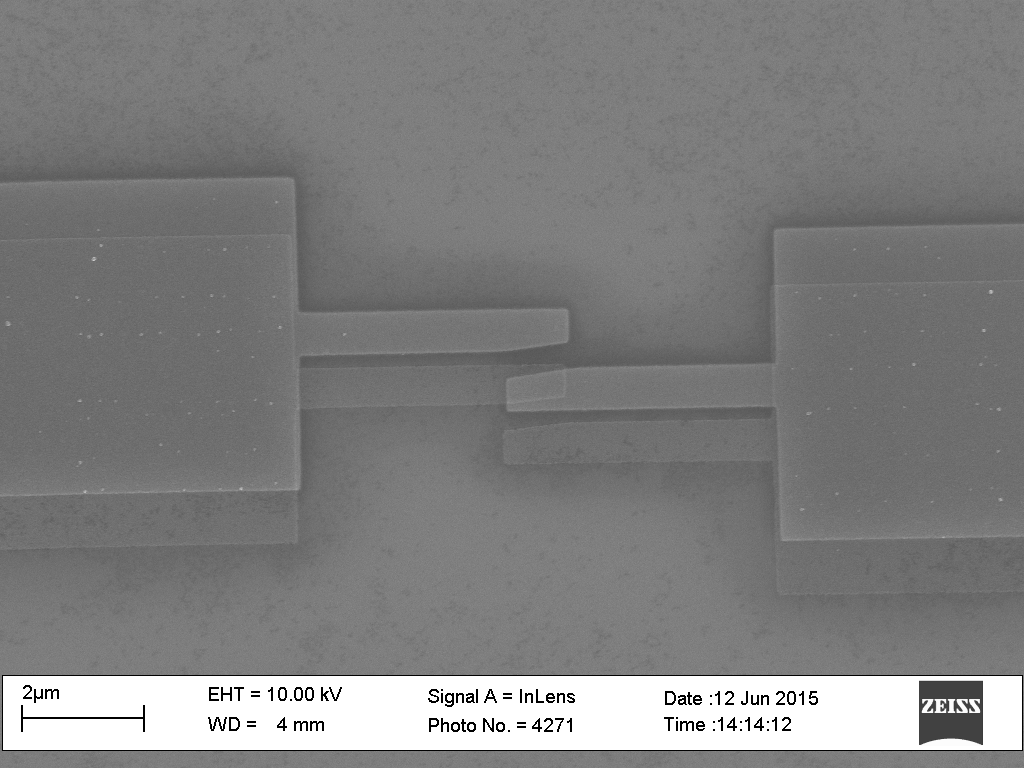
\includegraphics[width=6cm]{SEMtest12_1.png}
                    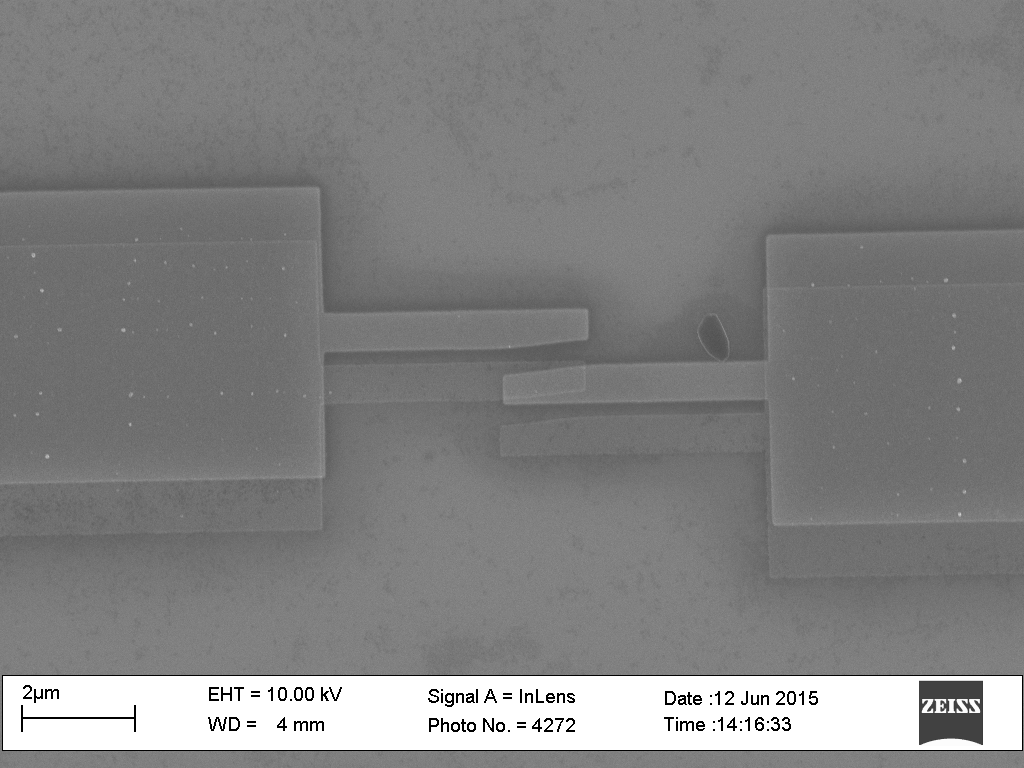
\includegraphics[width=6cm]{SEMtest12_2.png}
                    \caption{SEM images of the clean contact samples}
                    \label{SEMcleancontact}
                \end{figure}
                
                \begin{figure}
                    \centering
                    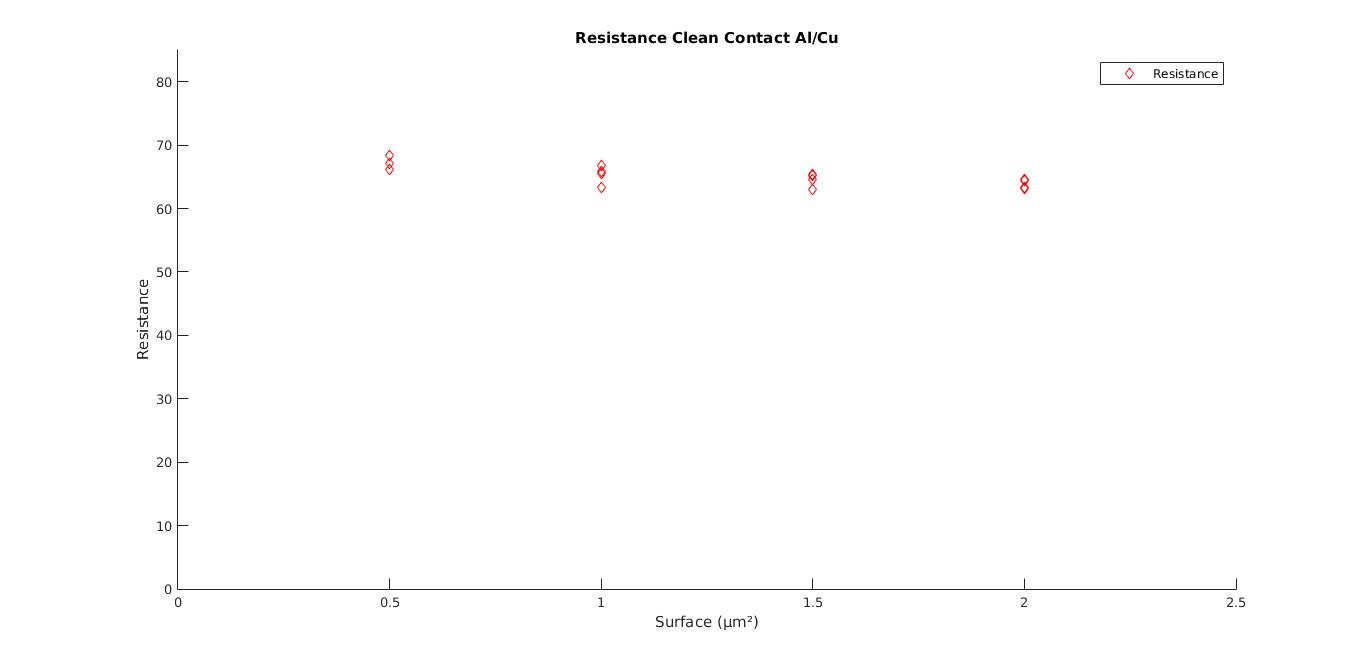
\includegraphics[width=12cm]{RClean.jpg}
                    \caption{Resistance of clean contact in function of the surface area}
                    \label{cleancontact}
                \end{figure}
                
                \subsection{Strong Oxidation}
                
                After the clean contact, I realized some reference samples for a strong oxidation, I oxidized freshly evaporated Al under a pressure of 200mbar during 10 minutes before evaporating Cu. The SEM images can be seen on Figure \ref{SEMstrongox}.
                
                \begin{figure}
                    \centering
                    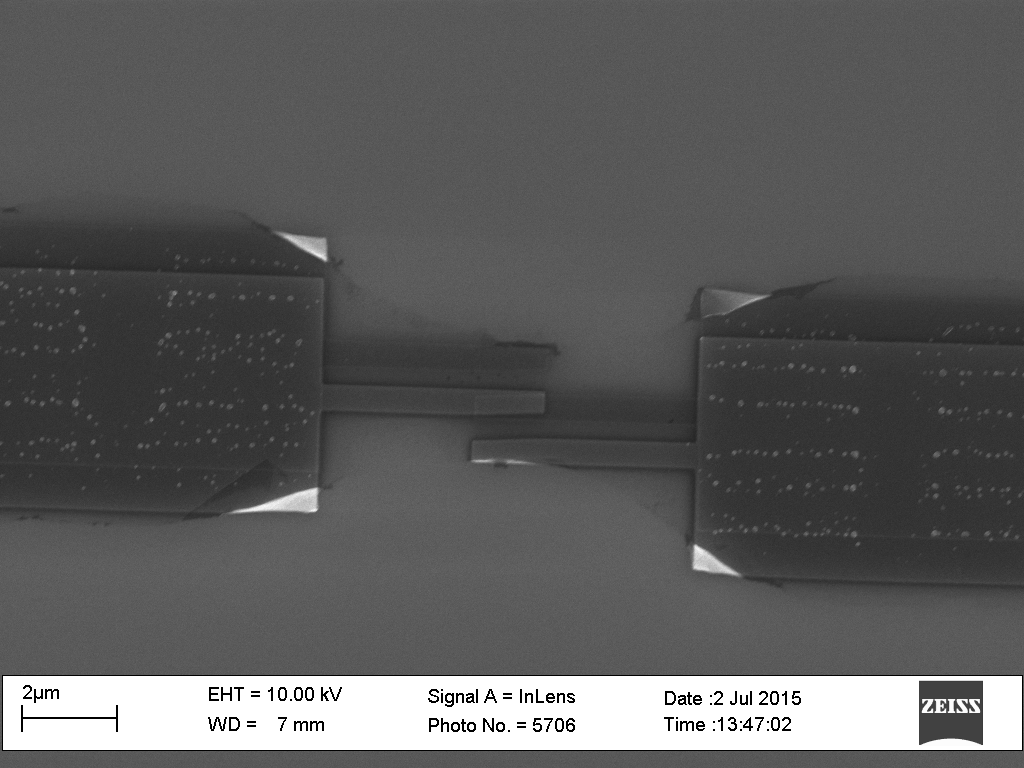
\includegraphics[width=6cm]{SEMtest15_1.png}
                    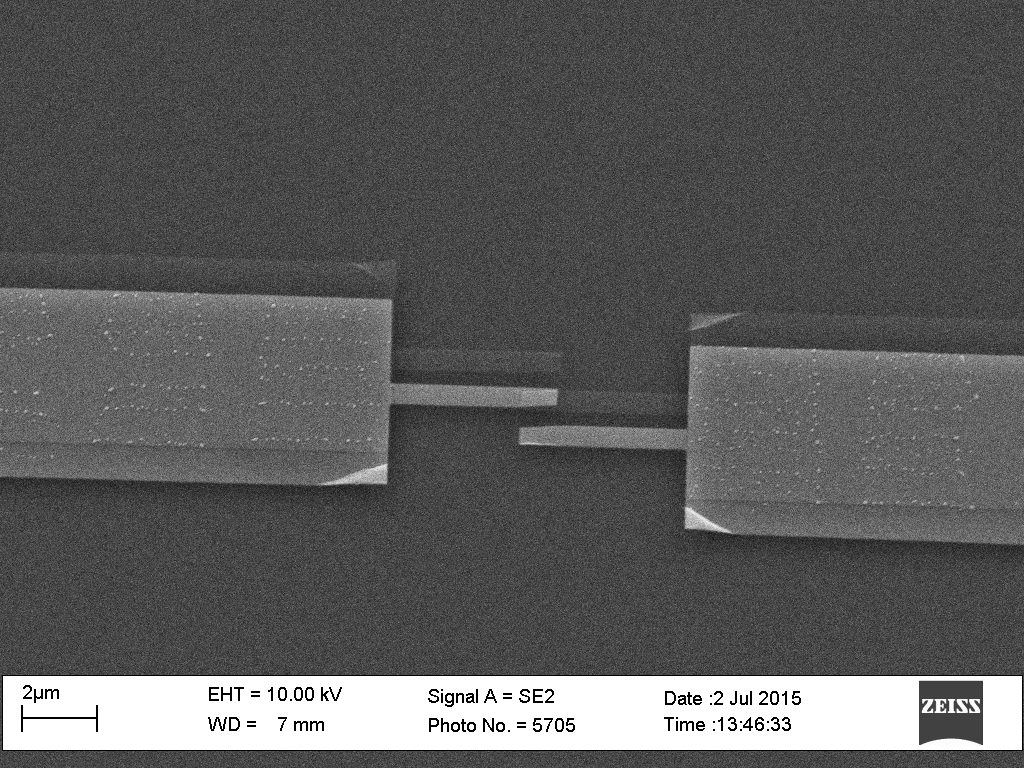
\includegraphics[width=6cm]{SEMtest15_2.png}
                    \caption{SEM images of the Strong Oxidation samples}
                    \label{SEMstrongox}
                \end{figure}
                
                For the NIS junctions, it is more relevant to draw conductance in function of the surface area of the junction so that we obtain a linear curve (See Fig. \ref{Strongox}), and we can determine the RS factor.
                
                \[RS=7.18k\Omega.\mu m^2\]
                
                \begin{figure}
                    \centering
                    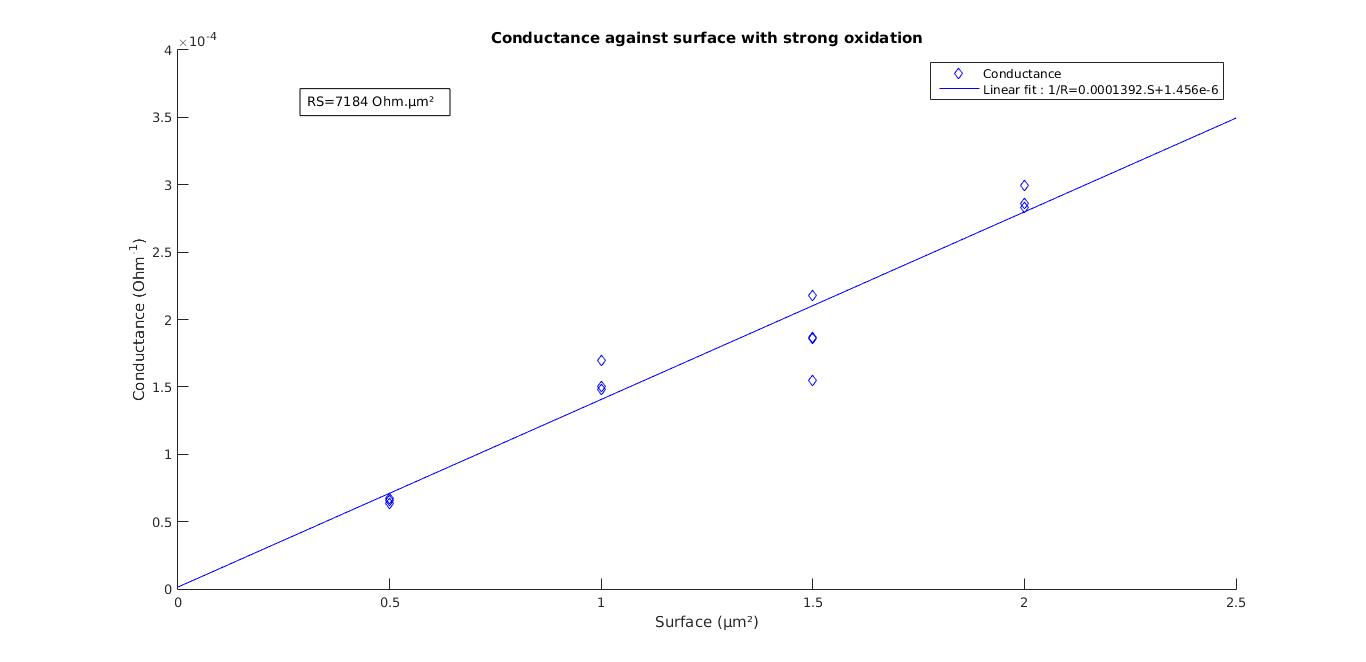
\includegraphics[width=12cm]{StrongOxLinear.jpg}
                    \caption{Conductance in function of surface area for a strong oxidized sample}
                    \label{Strongox}
                \end{figure}
                
                \section{Regular Oxidation}
                
                Then I have realized some samples with a regular oxidation to compare to the samples with the plasma. Here, I oxidize Al under 2mbar for 2 minutes before evaporating Cu.
                
                 \begin{figure}
                    \centering
                    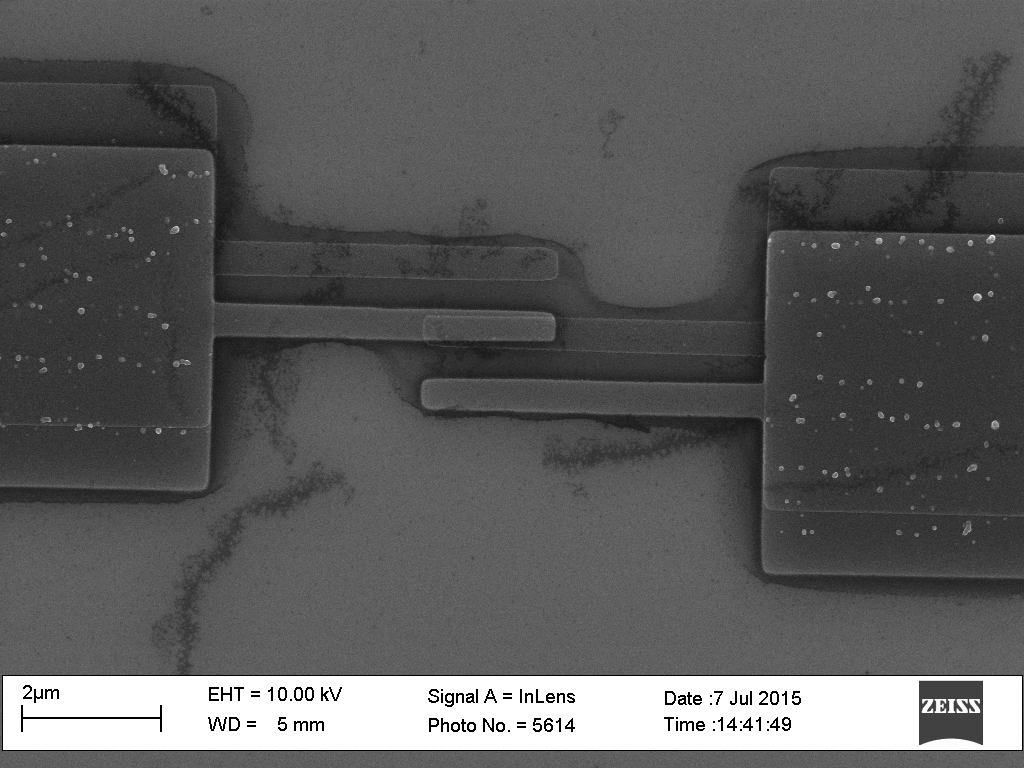
\includegraphics[width=6cm]{SEMtest16_1.png}
                    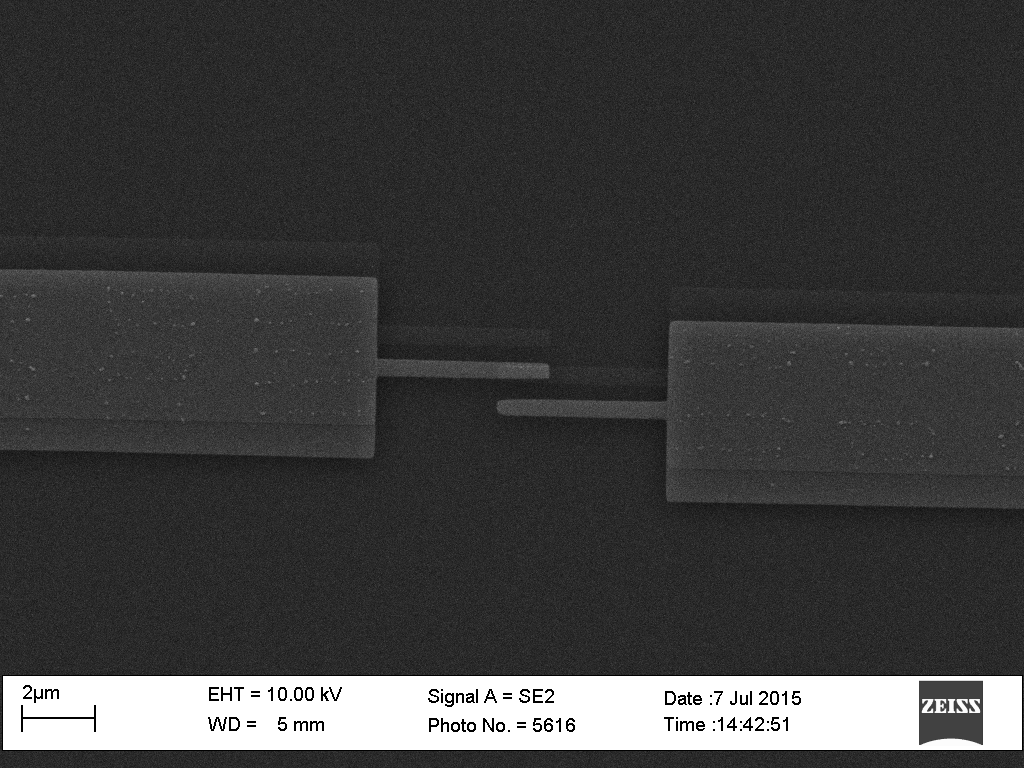
\includegraphics[width=6cm]{SEMtest16_2.png}
                    \caption{SEM images of the Regular Oxidation samples}
                    \label{SEMregularox}
                \end{figure}
                
                Again, it is more relevant to draw the conductance (See Fig. \ref{Regularox}) to determine the RS factor.
                
                \begin{figure}
                    \centering
                    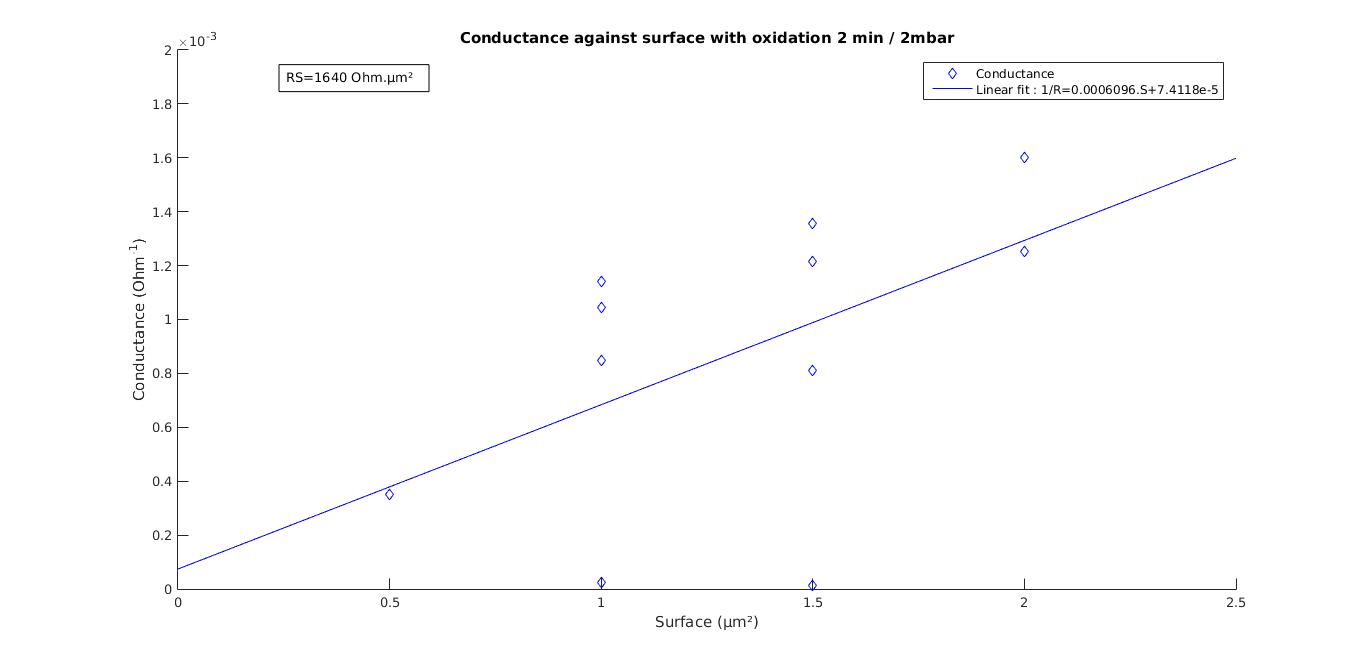
\includegraphics[width=12cm]{OxLinear.jpg}
                    \caption{Conductance in function of surface area for a regular oxidized sample}
                    \label{Regularox}
                \end{figure}
                                
                \[RS=1.64k\Omega.\mu m^2\]
                
                These junction are less resistive than the strong oxidation junction, which is normal because the thickness of the oxide is lower, so more electrons can go through the oxide.
                
                \subsection{Time of plasma}
                
                The time during which the sample is exposed to the plasma is important and determine how much oxide will be etched and implicitely the resistance of the sample.
                 In Figure \ref{SEMPlasma} there are some good samples made with plasma etching. Some samples also turned out to become failures, there are SEM images with explanation in Appendix \ref{badplasma}.
                 
                 
                 The Figure \ref{PlasmaTime} shows the resistance compared to plasma etching duration, so that we can roughly evaluate the thickness of the oxide.
                
                
                \subsection{Position of the sample}
                
                Then, I wanted to check if the plasma is uniform. We do not know if it affects equally all the areas of the sample stage or not. This is why I've made several tests where I placed 4 samples on the sample stage and did the evaporation. The Figure \ref{PlasmaPosition} shows the results of these tests. We can see that the position does not affect much the resistance of the sample so we can assume that the etching is quite uniform.
                
                
                \section{Low temperature measurements}
                
                \subsection{NIS Junction}
                
                Thanks to the dilution cryostat I was able to cool down some samples down to 50mK. Of course the pads on the sample stage are in a limited number so that I had to chose the best samples to bound and to cool down.
                
                
                
                \subsection{Plasma etched samples}
                
                
                
                \section{Summary of the results}
                
                
                
                
        
                
                
                
                
                
                
        
